\section{Results}
\label{sec:results}
In the next sections, I present the main results of my experiment to support our claim that SafraFT is correct, to show how SafraFT compares to SafraFS and to exemplify the performance of SafraFT under the presence of faults.

The observations are based on runs of the system described in \cref{sec:methods} on the DAS-4 cluster at the Vrije Universiteit of Amsterdam.
I measured runs on networks from 50 to 2000 nodes for SafraFT and SafraFS.
SafraFT was also tested with 1 to 5 nodes failing per run (dubbed 5n) and with 90\% node failure.
\cref{table:runs} presents how many repetitions of each configuration were run.

The raw data including a manual on how to interpret it can be found TODO here.
\begin{table}[]
	\centering
	\begin{tabular}{@{}llrrr@{}}
		\toprule
		Algorithm & Network              & Faults & Repetitions  & \#Instances / DAS-4 node   \\ \midrule
		SafraFS on CM and AKY  & 50/250/500/1000      & 0      & 50          & 50                    \\
		SafraFS on CM and AKY  & 2000                 & 0      & 50          & 100                   \\
		SafraFT on CM and AKY  & 50/250/500/1000      & 0      & 50          & 50                    \\
		SafraFT on CM and AKY  & 2000                 & 0      & 50          & 100                   \\
		SafraFT on CM and AKY  & 50/250/500/1000      & 5n     & 50          & 50                    \\
		SafraFT on CM and AKY  &    2000              & 5n     & 50          & 100                   \\
		SafraFT on CM and AKY  & 50/250/500/1000/     & 90\%   & 50          & 50                    \\
		SafraFT on CM and AKY  &    2000              & 90\%   & 50          & 100                   \\ \bottomrule
	\end{tabular}
	\caption{List of all configurations run. Per physical DAS-4 node with 8 cores multiple multiple virtual instances in their own processes where run (columm '\#Instances / DAS-4 node`). The amount of physical node equates to network size divided by instances.}
	\label{table:runs}
\end{table}

The results of runs with CM or AKY are quite similar and mostly show the same effect on the metrics.
Therefore, I analyse both together and explicitly state if an observation or explanation only applies to one of both.

\subsection{Correctness of SafraFT}
\label{ssec:correctness}
The experiment is aimed to support our paper with a practical, correct application of our algorithm.
Towards this goal, I build multiple correctness checks into the experiment.

To assure nothing happens after termination detection, the application logs if any messages are received or actions are executed after termination has been detected and announced.
The analysis tools provided with the experiment point these logs out to make sure they are not overlooked.

To proof termination is not detected too early, I use offline analysis (see \cref{ssec:offline-analysis}) to determine the point of actual termination and verify that detection happened after.
All 1000 runs using SafraFT under the presence of faults confirm that termination was never detected too early.
% NUMBER

However, the experiment revealed that the framework for termination chosen to develop SafraFT is not complete and does not cover all cases for my experimental setup.
SafraFT is developed for the following and commonly used definition of termination:
\begin{enumerate}
	\item All nodes are passive
	\item No messages are in the channels
\end{enumerate}
This definition is based on the fact that a node is either an initiator or can only become active if it receives a message.
Anyhow, in the presence of failures and if additionally, the outcome of the algorithm depends on the set of alive nodes, nodes might get activated by the detection of a failure.
For example, when Chandy Misra builds a sink tree, nodes that detect a crash of their parents will become active afterwards to find a new path towards the root.
This fact leads to the following concrete scenario in which the definition of termination assumes termination too early: let us consider the situation that all nodes are passive and no messages are in the channel.
In other words, the system terminated by our definition.
Node \co{X} forwards the token to \co{Y} and crashes afterwards.
Node \co{Y} calls announce after receipt of the token.
Assume node \co{Z} is a child of \co{X} and detects the crash of its parent, it becomes active after termination has been formally reached and announced.
By sending out \co{REQUEST} messages, it might activate other nodes again.
To conclude, the definition of termination that our algorithm is built upon does not fully capture the reality of our basic algorithms which could lead to an early detection of termination.

I propose an extended definition of termination to close this gap between theory and practice:
\begin{enumerate}
	\item All nodes are passive
	\item No messages are in the channels
	\item Termination is postponed until the last node failure that leads to action is detected
\end{enumerate}
\label{extended-definition}
All repetitions of this experiment have been analysed according to the common definition of termination used to develop SafraFT and the extended definition.
As stated above, SafraFT did never detect termination too early according to its definition.
According to the extended definition, it detects termination to early in \OutputFileNum{figures/early-termination.txt} out 1500 runs.  % NUMBER NUMBER
However, due to the fact that repairing the constructed trees after detecting a parent crash is quite fast and there is a short time window to do so while the announce call propagates to all nodes, only in \OutputFileNum{figures/early-termination-corrupted.txt} of these cases that leads to the situation that basic activity happened after detected termination. % NUMBNER


I carefully reviewed each repetition in which termination is detected too early according to the extended definition to verify that early termination detection is in fact caused by a situation as described above.
The logs of these runs provide a summary of all detections of parent crashes close to the announce call to ease this procedure.

\subsection{Comparision of Safra versions}
This section compares SafraFS and SafraFT.
Additionally, it analysis how the network size influences both algorithms.

The number of tokens sends in total and after termination is presented in \cref{fig:tokens-and-tokens-after-aky} for CM and in \cref{fig:tokens-and-tokens-after-aky} for AKY.

\begin{sidewaysfigure}[ht]
	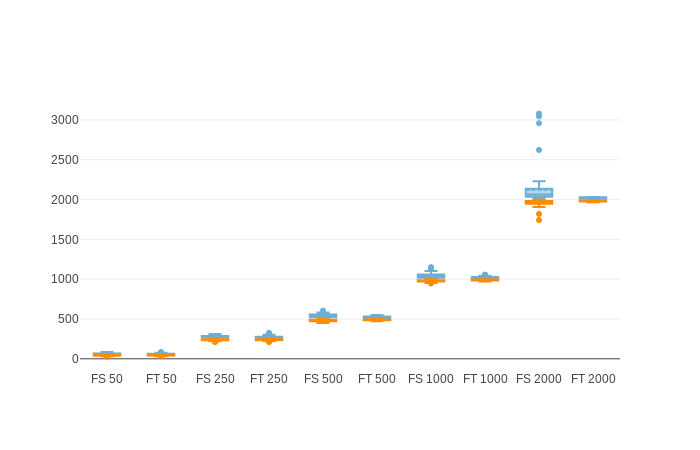
\includegraphics{figures/tokens-and-tokens-after-cm.png}
	\caption{Tokens (blue) and tokens after termination (orange) for SafraFT and SafraFS in fault free runs for all network sizes with the basic algorithm Chandy-Misra.}
	\label{fig:tokens-and-tokens-after-cm}
\end{sidewaysfigure}

%\begin{sidewaysfigure}[ht]
%    \includegraphics{figures/tokens-and-tokens-after-aky.png}
%    \caption{Tokens (blue) and tokens after termination (orange) for SafraFT and SafraFS in fault free runs for all network sizes with the basic algorithm Afek-Kutten-Yung.}
%    \label{fig:tokens-and-tokens-after-aky}
%\end{sidewaysfigure}
% TODO add figure


The key observation is that SafraFS and SafraFT behave highly similar.
SafraFT sends slightly fewer tokens on average.
Also, its results show less variance.
Most likely these differences are caused by implementation details and are not generalizable.

As one would expect, the number of tokens grows linearly with the network size.
Note that the first network size is 5 times smaller than the second for bigger networks the size doubles for each run.

The same can be observed for tokens sent after termination.
By far most tokens are sent after termination as one would expect.

The bit complexity of SafraFS is constant.
In this experiment, each token of SafraFS contains 12 bytes.
SafraFT has a bit complexity linearly to the network size (when no faults occur).
For a network of 50 nodes, each token has 220 bytes; a token in a 2000 node network counts 8020 bytes.
The growth can be described by $bytes = 4 * <network size> + 20$.

I measured two kinds of timing metrics in this experiment.
On the one hand, there are the wall time metrics of total time and total time after termination.
Both were recorded in elapsed seconds between two events.
For the total time, these events are the start of the basic algorithm and termination detection event at the last node.
Total time after termination is defined as the number of seconds between the actual termination (extended termination definition from \cref{ssec:correctness}) and the event of a node calling
announce.
On the other hand, there are basic, Safra and Safra after termination processing times (including the time needed to send messages).
These are the accumulated times all instances needed to process basic or Safra functions.
Total times and processing times are measured in a different way and should not be compared directly for multiple reasons.
First, while total times include idle times, e.g. time spent for logging, processing time do not include these.
Secondly, total time is wall time between two events and processing times are accumulated over all processes.
One particular example of when this leads to differences is that time spent concurrently by two processes counts double in processing time metrics but only once in wall time metrics.

\begin{table}
	\centering
	\begin{tabular}{rrrrrr||rr}%
		\toprule
		\multicolumn{1}{c}{Network} &
		\multicolumn{1}{c}{Basic} &
		\multicolumn{1}{c}{Safra FS} &
		\multicolumn{1}{c}{Safra FT} &
		\multicolumn{1}{c}{Overhead FS} &
		\multicolumn{1}{c||}{Overhead FT} &
		\multicolumn{1}{c}{Safra FS}   &
		\multicolumn{1}{c}{Safra FT}
		\\
		\midrule
		\csvreader[head to column names]{figures/processing-times-cm.csv}{}
		{\\\networkSize & \basic & \FS & \FT  & \FSoverhead \% & \FToverhead \% & \FSAfter & \FTAfter}
		\\\bottomrule
	\end{tabular}
	\caption{Total processing times (left) and processing times after termination (right) in seconds and overhead over Chandy-Misra caused by Safra in percent}
	\label{table:processing-times-cm}
\end{table}

\begin{table}
	\centering
	\begin{tabular}{rrrrrr||rr}%
		\toprule
		\multicolumn{1}{c}{Network} &
		\multicolumn{1}{c}{Basic} &
		\multicolumn{1}{c}{Safra FS} &
		\multicolumn{1}{c}{Safra FT} &
		\multicolumn{1}{c}{Overhead FS} &
		\multicolumn{1}{c||}{Overhead FT} &
		\multicolumn{1}{c}{Safra FS}   &
		\multicolumn{1}{c}{Safra FT}
		\\
		\midrule
		\csvreader[head to column names]{figures/processing-times-aky.csv}{}
		{\\\networkSize & \basic & \FS & \FT  & \FSoverhead \% & \FToverhead \% & \FSAfter & \FTAfter}
		\\\bottomrule
	\end{tabular}
	\caption{Total processing times (left) and processing times after termination (right) in seconds and overhead over Afek-Kutten-Yung caused by Safra in percent}
	\label{table:processing-times-aky}
\end{table}

One can observe in \cref{table:processing-times-cm} and \cref{table:processing-times-aky} that SafraFT uses more processing time than SafraFS and much of the additional time is spent between actual termination and termination detection.
The processing time increases linearly with the network size for SafraFS.
For SafraFT doubling the network size leads to a 2 or threefold increase in processing time.
Most of the additional processing time of SafraFT is spent between termination and termination detection.
One can also see that the processing time increased more than twofold for networks of 1000 nodes to 2000 nodes.
This is most likely due to the fact that 2000 node networks were simulated by running 100 instances instead of 50 instances per physical node.

A good candidate to explain the difference in processing time between SafraFS and SafraFT is the different token size of SafraFS and SafraFT: it takes longer to send bigger tokens.
Also, this theory is supported by the fact that most additional time is spent after termination - Safra is only concerned with moving the token around after termination.
To confirm this idea, I ran an ad-hoc experiment of excluding the time spent to send messages from the processing time.
Indeed, this experiment revealed that most of the differences can be tributed to writing tokens onto the wire.
Therefore, I believe that these differences are caused by the higher bit complexity of SafraFT.
This would explain the total increase in the timing from SafraFS to SafraFT, as well as, the bigger influence of network size - bigger networks lead to even larger tokens.

The qualitative result is not surprising.
However, we are surprised by the quantitative size it has.
We would have expected that the difference between SafraFS and SafraFT in processing time is observable but much lower.
A possible explanation can be found in my experiment setup: each physical node simulates between 50 and 100 instances.
Each of this instances uses multiple threads; altogether there are at least 4 times as many threads as cores on each machine.

The huge quantitative effect could in part be caused by threads being preempted which happens more often for threads that try to send big messages.
This theory is supported by the fact that the effect is stronger for networks with 2000 nodes.
However, confirmation of that assumption is not in the scope of this project.

The processing time \cref{table:processing-times} also presents a comparison of the time spent on the basic algorithm and both Safra versions.
Although SafraFT uses significantly more time, the overhead on the processing time stays moderate with a maximum of NUMBER for 2000 nodes and AKY.
% NUMBER



\begin{table}
	\centering
	\begin{tabular}{rrrr||rrr}%
		\toprule
		\multicolumn{1}{c}{Network} &
		\multicolumn{1}{c}{Safra FS} &
		\multicolumn{1}{c}{Safra FT} &
		\multicolumn{1}{c||}{$\Delta$} &
		\multicolumn{1}{c}{SafraFS}  &
		\multicolumn{1}{c}{SafraFT}  &
		\multicolumn{1}{c}{$\Delta$}  \\
		\midrule
		\csvreader[head to column names]{figures/total-times-cm.csv}{}
		{\\\networkSize & \FS & \FT & \difference & \FSAfter & \FTAfter & \differenceAfter}
		\\\bottomrule
	\end{tabular}
	\caption{Wall times total (left) and after termination (right) for SafraFT and SafraFS in seconds with ratios run with CM}
	\label{table:total-times-cm}
\end{table}

\begin{table}
	\centering
	\begin{tabular}{rrrr||rrr}%
		\toprule
		\multicolumn{1}{c}{Network} &
		\multicolumn{1}{c}{Safra FS} &
		\multicolumn{1}{c}{Safra FT} &
		\multicolumn{1}{c||}{$\Delta$} &
		\multicolumn{1}{c}{SafraFS}  &
		\multicolumn{1}{c}{SafraFT}  &
		\multicolumn{1}{c}{$\Delta$}  \\
		\midrule
		\csvreader[head to column names]{figures/total-times-aky.csv}{}
		{\\\networkSize & \FS & \FT & \difference & \FSAfter & \FTAfter & \differenceAfter}
		\\\bottomrule
	\end{tabular}
	\caption{Wall times total (left) and after termination (right) for SafraFT and SafraFS in seconds with ratios run with AKY}
	\label{table:total-times-aky}
\end{table}

The same pattern of SafraFT using more time and reacting stronger to an increase in network size is visible for total times in \cref{table:total-times-cm} and \cref{table:total-times-aky} for CM and AKY respectively.

For SafraFS and CM, roughly half of the time is spent after termination for small networks.
In big networks, the part of the time spent after termination is lower because the fraction spent by the basic algorithm becomes dominant.
The systems using SafraFT spent half or more of their time to detect termination.

For AKY most of the time is spent before termination (except for 1000 and 2000 nodes and SafraFT).
This shows that the time measurements highly depend on the basic algorithm.
AKY is a synchronized algorithm and needs more time than CM.

I would like to note that the low processing time overhead of Safra is not in contradiction to a large amount of wall time spent after termination.
These seemingly opposing results arise from the difference between wall time and processing time: the basic algorithm is much more active at the beginning that is when it accumulates a lot of processing time; while Safra causes a lot of idle time in the end when all processes wait for their predecessor to pass on the token.
This idle time is not included in processing time but wall time does include it.

To conclude, the experiments confirm that the message complexity of SafraFT remains as for the fault sensitive version but its higher bit complexity causes it to use more time which leads to a later termination detection.
Still, SafraFT causes only a moderate processing time overheads between NUMBER and NUMBER. % NUMBER

\subsection{Influence of faults}
In the following paragraphs, I present and explain the data generated by runs in the presence of node crashes.
I run two highly different scenarios: one considering networks with 1 to 5 nodes failing and one with 90\% of all nodes crashing.
These scenarios are chosen to show SafraFT in both the realistic case of a low number of faults to handle, as well as, an extreme case; with the aim to confirm that SafraFT handles both cases correctly and without unreasonable deterioration in any metric.

I used the extended definition of termination to determine the point of time of actual termination to generate the metrics shown in this section.

\subsubsection{Tokens}
\label{ssec:tokens-faulty}
For both the networks where between 1 and 5 nodes failed, as well as, for the highly faulty runs with 90\% node failure, the number of tokens increased compared to runs without any faults.
Runs with 90\% failure produced even more tokens than runs with only 1 to 5 node failing - except in networks of 2000 nodes where 5n exhibits a higher token sent average.
The data is presented~\cref{fig:tokens-and-tokens-after-faulty-cm}~/~\ref{fig:tokens-and-tokens-after-faulty-aky} and~\cref{table:tokens-faulty-cm}~/~\ref{table:tokens-faulty-aky} for CM respectively AKY.

\begin{sidewaysfigure}[ht]
	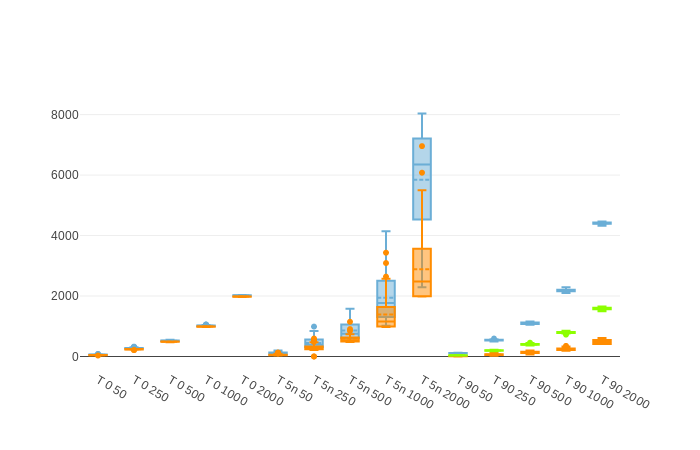
\includegraphics{figures/tokens-and-tokens-after-faulty-cm.png}
	\caption{SafraFT and CM: Tokens (blue) and tokens after termination (orange) for SafraFT on the x-axis for 5 network sizes and 5n and 90\% fault configurations on the y-axis.        Backup tokens in green, shown only for 90\%}
	\label{fig:tokens-and-tokens-after-faulty-cm}
\end{sidewaysfigure}

%\begin{sidewaysfigure}[ht]
%    \includegraphics{figures/tokens-and-tokens-after-faulty-aky.png}
%    \caption{SafraFT and AKY: Tokens (blue) and tokens after termination (orange) for SafraFT on the x-axis for 5 network sizes and 5n and 90\% fault configurations on the y-axis.        Backup tokens in green, shown only for 90\%}
%    \label{fig:tokens-and-tokens-after-faulty-aky}
%\end{sidewaysfigure}
% TODO add figure


\begin{table}
	\centering
	\begin{tabular}{rrrrrr||rrrrr}%
		\toprule
		\multicolumn{1}{c}{Network} &
		\multicolumn{1}{c}{No faults} &
		\multicolumn{1}{c}{5n} &
		\multicolumn{1}{c}{$\Delta$} &
		\multicolumn{1}{c}{90\%} &
		\multicolumn{1}{c||}{$\Delta$} &
		\multicolumn{1}{c}{No faults} &
		\multicolumn{1}{c}{5n} &
		\multicolumn{1}{c}{$\Delta$} &
		\multicolumn{1}{c}{90\%} &
		\multicolumn{1}{c}{$\Delta$} \\
		\midrule
		\csvreader[head to column names]{figures/tokens-faulty-cm.csv}{}
		{\\\networkSize & \noFaults & \fiveN & \differenceFiveN & \ninety & \differenceNinety &
		\noFaultsAfter & \fiveNAfter & \differenceFiveNAfter & \ninetyAfter & \differenceNinetyAfter }
		\\\bottomrule
	\end{tabular}
	\caption{SafraFT and CM: Tokens in total (left) and after termination (right) for different fault scenarios compared to fault-free networks.}
	\label{table:tokens-faulty-cm}
\end{table}

\begin{table}
	\centering
	\begin{tabular}{rrrrrr||rrrrr}%
		\toprule
		\multicolumn{1}{c}{Network} &
		\multicolumn{1}{c}{No faults} &
		\multicolumn{1}{c}{5n} &
		\multicolumn{1}{c}{$\Delta$} &
		\multicolumn{1}{c}{90\%} &
		\multicolumn{1}{c||}{$\Delta$} &
		\multicolumn{1}{c}{No faults} &
		\multicolumn{1}{c}{5n} &
		\multicolumn{1}{c}{$\Delta$} &
		\multicolumn{1}{c}{90\%} &
		\multicolumn{1}{c}{$\Delta$} \\
		\midrule
		\csvreader[head to column names]{figures/tokens-faulty-aky.csv}{}
		{\\\networkSize & \noFaults & \fiveN & \differenceFiveN & \ninety & \differenceNinety &
		\noFaultsAfter & \fiveNAfter & \differenceFiveNAfter & \ninetyAfter & \differenceNinetyAfter }
		\\\bottomrule
	\end{tabular}
	\caption{SafraFT and AKY: Tokens in total (left) and after termination (right) for different fault scenarios compared to fault-free networks.}
	\label{table:tokens-faulty-aky}
\end{table}

Otherwise, the two types of fault simulation have a highly different influence on the tokens and tokens after termination metrics.

5n configurations lead to a strong increase in the variance of tokens sent and in tokens sent after termination.
This seems reasonable because runs with failing nodes might lead to more different situations as runs without fails e.g. one failing node could easily cause an extra token round when it leads to a backup token being issued and forwarded (this token is marked black until it reaches the node it originates from), at the same time, a single failing node that is a leaf in a Chandy Misra sink tree and that crashes just before the call of announcing at the successor  causes no further activity.
The same example provides an idea of why the variability increases in big networks.
That is because one extra round in a big network has a much higher impact on the token count than in a small network.

Opposed to the results for 5n, networks with up to 90\% node failure lead to a similar low variance in tokens and tokens after termination as fault-free networks.
A likely explanation is that the low survival rate of 1 out of 10 instances leads to less different scenarios than in the fault scenario treated in the last paragraphs.

Even though only one 10th of the nodes survive to participate in the latter token rounds, the highly faulty networks produced more tokens than any other network of the same size.
That is most likely due to the high amount of backup tokens generated (also shown in \cref{fig:tokens-and-tokens-after-faulty})

Different from all other networks, highly faulty networks exhibit a much lower token to token after termination ratio caused by the low number of nodes alive in the last rounds.

As expected, faults lead to more token being sent.
This is caused mostly because a fault detection requires an additional round.
However, SafraFT handles faults kindly - neither 5n nor 90\% scenarios lead to an overhead higher than 2.13 compared to a fault-free execution.
Hence, not every fault causes an extra round but all faults together cost an extra round.
This result holds for all network sizes, both basic algorithm and for two highly different fault scenarios.

\subsubsection{Backup tokens}
The average amount of backup tokens sent for either fault simulation or network size is lower than the number of faults.
This is due to the fact that SafraFT only issues backup tokens when the fault of its successor is detected via the fault detector but not if this fault is noticed by receiving a token.
There are even runs where 1 to 5 nodes fail but no backup token is issued up to networks containing 2000 nodes.

The other extreme that more backup tokens, than faults occur, are issued exists as well.
This can be explained by my decision to have node failing after issuing a backup token.
For example, nodes \co{A}, \co{B} and \co{C} follow each other in the ring, node \co{C} fails which is detected by \co{B} and a backup token is issued.
After, issueing the backup token \co{B} fails on detection \co{A} issues a backup token towards \co{C}.
Only then \co{A} detects the failing of \co{C} and issues a second backup token to its new successor.

Although both extremes exist, the average amount of backup token is close to the number of faulty nodes.

\subsubsection{Token size}
\begin{table}
	\centering
	\begin{tabular}{rrrrrr}%
		\toprule
		\multicolumn{1}{c}{Network} &
		\multicolumn{1}{c}{No faults} &
		\multicolumn{1}{c}{5n} &
		\multicolumn{1}{c}{$\Delta$} &
		\multicolumn{1}{c}{90\%} &
		\multicolumn{1}{c}{$\Delta$}  \\
		\midrule
		\csvreader[head to column names]{figures/token-sizes-faulty-cm.csv}{}
		{\\\networkSize & \noFaults & \fiveN & \differenceFiveN & \ninety & \differenceNinety }
		\\\bottomrule
	\end{tabular}
	\caption{SafraFT and CM: Token size averages in bytes for both fault scenarios compared to token size with zero faults.}
	\label{table:token-sizes-faulty-cm}
\end{table}

\begin{table}
	\centering
	\begin{tabular}{rrrrrr}%
		\toprule
		\multicolumn{1}{c}{Network} &
		\multicolumn{1}{c}{No faults} &
		\multicolumn{1}{c}{5n} &
		\multicolumn{1}{c}{$\Delta$} &
		\multicolumn{1}{c}{90\%} &
		\multicolumn{1}{c}{$\Delta$}  \\
		\midrule
		\csvreader[head to column names]{figures/token-sizes-faulty-aky.csv}{}
		{\\\networkSize & \noFaults & \fiveN & \differenceFiveN & \ninety & \differenceNinety }
		\\\bottomrule
	\end{tabular}
	\caption{SafraFT and AKY: Token size averages in bytes for both fault scenarios compared to token size with zero faults.}
	\label{table:token-sizes-faulty-aky}
\end{table}

The average token size increases with faults because the IDs of faulty nodes are propagated by the token (see~\cref{table:token-sizes-faulty} and~\ref{table:token-sizes-faulty-aky}).
The influence on token size is between 5 and 8 bytes for networks with 1 to 5 failing nodes.  % NUMBER
90\% node failure leads to a linear increase of token bytes to the network size of a factor 1.29. % NUMBER


\subsubsection{Processing Time}
The observations of this chapter are backed by \cref{table:processing-times-faulty-cm} and \ref{table:processing-times-aky}.
As for tokens, one can see an increase in total processing times under the presence of faults compared to fault-free runs which is no surprise because more tokens are sent.
This also explains why the processing time is higher for the 90\% scenario than in the 5n configurations.
There is one exception: the processing time for 2000 nodes and AKY in the 5n scenario decreased.

Processing times after termination for 90\% drastically decreased for both algorithm and all network sizes - except for CM and 50 nodes where one sees a 20\% increase.
The general result can be explained by fewer tokens being sent after termination.
The exception cannot be explained with the data at hand because it does only occur for one algorithm.

The influence of 5n scenarios on processing time after termination is highly varied.
In many configurations, it shows no big effect e.g. 250 nodes and CM.
In others, it decreases significantly e.g. 1000 and AKY.
And finally, one observes a sharp increase for 50 or 2000 and CM.
The available data does not allow for a good explanation.
One highly interesting fact is that 5n scenarios lead to more token being sent after termination (see \cref{table:tokens-faulty-cm} and \ref{table:tokens-faulty-aky}) but to less processing time after termination in many configurations.
This situation might be explained by the fact that the sum of all token counters is calculated by most nodes if no nodes failed and only by some nodes when other nodes crashed - due to the different \textit{blackUntil} values.

\begin{table}
	\centering
	\begin{tabular}{rrrrrr||rrrrr}%
		\toprule
		\multicolumn{1}{c}{Network} &
		\multicolumn{1}{c}{No faults} &
		\multicolumn{1}{c}{5n} &
		\multicolumn{1}{c}{$\Delta$} &
		\multicolumn{1}{c}{90\%} &
		\multicolumn{1}{c||}{$\Delta$} &
		\multicolumn{1}{c}{No faults} &
		\multicolumn{1}{c}{5n} &
		\multicolumn{1}{c}{$\Delta$} &
		\multicolumn{1}{c}{90\%} &
		\multicolumn{1}{c}{$\Delta$} \\
		\midrule
		\csvreader[head to column names]{figures/processing-times-faulty-cm.csv}{}
		{\\\networkSize & \noFaults & \fiveN & \differenceFiveN & \ninety & \differenceNinety &
		\noFaultsAfter & \fiveNAfter & \differenceFiveNAfter & \ninetyAfter & \differenceNinetyAfter }
		\\\bottomrule
	\end{tabular}
	\caption{SafraFT and CM: Total processing times (left) and after termination (right) in seconds for different fault scenarios compared to fault-free networks.}
	\label{table:processing-times-faulty-cm}
\end{table}

\begin{table}
	\centering
	\begin{tabular}{rrrrrr||rrrrr}%
		\toprule
		\multicolumn{1}{c}{Network} &
		\multicolumn{1}{c}{No faults} &
		\multicolumn{1}{c}{5n} &
		\multicolumn{1}{c}{$\Delta$} &
		\multicolumn{1}{c}{90\%} &
		\multicolumn{1}{c||}{$\Delta$} &
		\multicolumn{1}{c}{No faults} &
		\multicolumn{1}{c}{5n} &
		\multicolumn{1}{c}{$\Delta$} &
		\multicolumn{1}{c}{90\%} &
		\multicolumn{1}{c}{$\Delta$} \\
		\midrule
		\csvreader[head to column names]{figures/processing-times-faulty-aky.csv}{}
		{\\\networkSize & \noFaults & \fiveN & \differenceFiveN & \ninety & \differenceNinety &
		\noFaultsAfter & \fiveNAfter & \differenceFiveNAfter & \ninetyAfter & \differenceNinetyAfter }
		\\\bottomrule
	\end{tabular}
	\caption{SafraFT and AKY: Total processing times (left) and after termination (right) in seconds for different fault scenarios compared to fault-free networks.}
	\label{table:processing-times-faulty-aky}
\end{table}


\subsubsection{Total time}
Total time in faulty networks is presented in \cref{table:total-times-faulty} and \ref{table:total-times-aky}.
In line with the observations from the processing time section, one observes:
\begin{itemize}
	\item an increase in total time spent on fault scenarios
	\item less time spent after termination by highly faulty networks - except for 50 nodes and CM
	\item varied results for 5n scenarios and time spent after termination
\end{itemize}

\begin{table}
	\centering
	\begin{tabular}{rrrrrr||rrrrr}%
		\toprule
		\multicolumn{1}{c}{Network} &
		\multicolumn{1}{c}{No faults} &
		\multicolumn{1}{c}{5n} &
		\multicolumn{1}{c}{$\Delta$} &
		\multicolumn{1}{c}{90\%} &
		\multicolumn{1}{c||}{$\Delta$} &
		\multicolumn{1}{c}{No faults} &
		\multicolumn{1}{c}{5n} &
		\multicolumn{1}{c}{$\Delta$} &
		\multicolumn{1}{c}{90\%} &
		\multicolumn{1}{c}{$\Delta$} \\
		\midrule
		\csvreader[head to column names]{figures/total-times-faulty-cm.csv}{}
		{\\\networkSize & \noFaults & \fiveN & \differenceFiveN & \ninety & \differenceNinety &
		\noFaultsAfter & \fiveNAfter & \differenceFiveNAfter & \ninetyAfter & \differenceNinetyAfter }
		\\\bottomrule
	\end{tabular}
	\caption{SafraFT and CM: Total times (left) and after termination (right) in seconds. For different fault scenarios compared to fault-free networks.}
	\label{table:total-times-faulty-cm}
\end{table}

\begin{table}
	\centering
	\begin{tabular}{rrrrrr||rrrrr}%
		\toprule
		\multicolumn{1}{c}{Network} &
		\multicolumn{1}{c}{No faults} &
		\multicolumn{1}{c}{5n} &
		\multicolumn{1}{c}{$\Delta$} &
		\multicolumn{1}{c}{90\%} &
		\multicolumn{1}{c||}{$\Delta$} &
		\multicolumn{1}{c}{No faults} &
		\multicolumn{1}{c}{5n} &
		\multicolumn{1}{c}{$\Delta$} &
		\multicolumn{1}{c}{90\%} &
		\multicolumn{1}{c}{$\Delta$} \\
		\midrule
		\csvreader[head to column names]{figures/total-times-faulty-aky.csv}{}
		{\\\networkSize & \noFaults & \fiveN & \differenceFiveN & \ninety & \differenceNinety &
		\noFaultsAfter & \fiveNAfter & \differenceFiveNAfter & \ninetyAfter & \differenceNinetyAfter }
		\\\bottomrule
	\end{tabular}
	\caption{SafraFT and AKY Total times (left) and after termination (right) in seconds. For different fault scenarios compared to fault-free networks.}
	\label{table:total-times-faulty-aky}
\end{table}


